\section{The delayed-advice audit framework}\label{sec:framework}
\subsection{An executable evaluation procedure}
The framework turns the three questions into separate audit routes (Fig.~\ref{fig:workflow}; Algorithm~\ref{alg:audit}). Models, option functions and statistical comparisons are frozen before test environments are opened. Source competence is assessed separately from its marginal contribution at arrival. Local references include continued local control and development-selected fixed options; a hindsight-best option is never presented as executable assistance.
\begin{figure}[tb]\centering
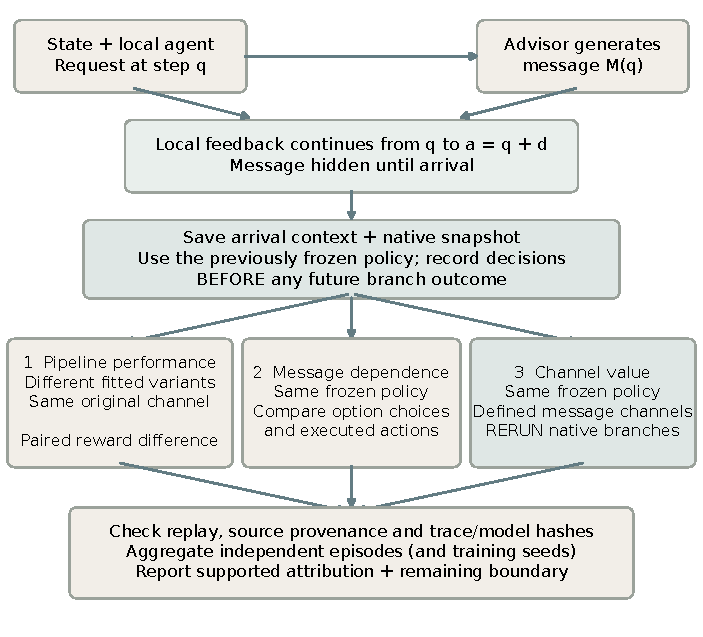
\includegraphics[width=\textwidth]{figures/advice_audit_workflow.pdf}
\caption{The delayed-advice audit workflow. Local control advances while a message is unavailable. At arrival, choices are logged before future outcomes. Pipeline comparisons use different fitted variants; dependence checks inspect choices and commands of a fixed policy; channel-value tests rerun actual native branches under defined message mechanisms. Replay and provenance checks precede attribution.}\label{fig:workflow}
\end{figure}
\begin{algorithm}[tb]
\caption{Delayed-Advice Audit Procedure}\label{alg:audit}
\small
\textbf{Inputs:} local controller, advisor, trained arrival policies, message channels, delay/query protocol, option functions, continuation, held-out environments and exogenous seeds.\par
\begin{enumerate}
\item Specify $U$, costs, $T$, splits, primary contrasts, uncertainty method, and the conditioning of each channel. Define missing-message behavior explicitly.
\item Fit/select only on development episodes, or reuse verified trained policies. Freeze weights, normalization, thresholds, option functions and source hashes.
\item For each held-out episode, run local control to $q$, generate the permitted request message, and continue locally to $a=q+d$ without exposing it early.
\item Save the arrival snapshot and permitted nonmessage context. Generate each control message only from its declared observation/time information.
\item For every frozen policy and channel, log inputs, message provenance, scores and the selected option \emph{before} any branch outcome is observed.
\item Restore the common snapshot and execute each required option/message branch through its repair window and common continuation to $T$. Reuse a trace only for an exactly identical executable plan. Evaluate all options only when an offline headroom diagnostic is declared.
\item Check complete replay, hashes, source-message consistency, trajectory lengths and agreement between saved choices, actions and rewards. Report failures instead of silently excluding episodes.
\item Estimate pipeline contrasts separately from fixed-policy channel contrasts. Record both decision and command changes. Resample complete environments and training seeds as required, not correlated option branches.
\item Report the supported attribution, channel/support/cost boundary and finite-pool diagnostics. If no outcome-valid channel intervention was executed, leave $\Delta_{\rm ch}$ unestimated.
\end{enumerate}
\textbf{Outputs:} auditable performance contrasts, dependence diagnostics, defined channel-value estimates where available, and a claim-boundary record.
\end{algorithm}

For a single arrival, compared branches share the request trajectory, fixed arrival context and future exogenous noise. Their intervened messages and option selections may differ. Each branch executes its actual native action rule and then returns to the same continuation controller. Complete episodes define train/validation/test groups and resampling units. Snapshots, branch rewards and native prefix success are excluded from policy features.

Counterfactual consistency requires restoring more than generalized coordinates. Our snapshot includes full MuJoCo integration and derived data, Python-side task state, observation history, reward bookkeeping, relevant model arrays, random state and aliases into native arrays. Copying an aliased view into a detached array can change reward semantics. Under the declared renderer, complete-tail checks compare images, predictions, actions, rewards and success labels. These checks establish local consistency, not universal simulator or hardware determinism.

\subsection{An executable null-advice certificate}\label{sec:null}
A zero gain predictor makes one dependency case inspectable. Let every nonreject option and reject have predicted gain zero, and intervene only when the selected gain exceeds a positive threshold. The deployed gate then always returns $R$.
\begin{proposition}\label{prop:null}
Suppose a frozen arrival policy always rejects and its continuing local controller does not consume returned messages. If queries do not affect physical transitions, observations or local-controller resources, replacing or removing the messages preserves every action and reward under the same initial state and exogenous randomness.
\end{proposition}
\begin{proof}
Before arrival, the histories and local actions agree. At arrival both implementations select $R$. Their next local actions agree, and coupled transition/observation functions give the same next histories. Induction through the remaining steps and any further scheduled arrivals proves equality.\qed
\end{proof}
An instrumented evaluator may still generate, serialize or normalize a packet before returning the zero decision. The certificate concerns functional action/reward dependence and an equivalent packet-free implementation, not an observed saving in message-processing time. This is a simple dependency argument, not a new control theorem. Real queries can consume shared compute or human attention, violating its assumptions. Our forced-query simulator does not measure such savings.

A finite example explains the attribution problem. In one known state, two executable local actions have rewards 0 and 1; the continuation chooses the latter. A fitted local-input variant mistakenly intervenes with the former, whereas a packet-input pipeline selects the zero predictor and rejects. Its pipeline advantage is 1 for any returned message, including an irrelevant constant, but the winning policy has no runtime message dependence. A positive $\Delta_{\rm pipe}$ is therefore compatible with zero channel effect. The implemented visual study tests whether this possibility occurs in an actual learning pipeline.

\subsection{Diagnosing opportunity and selection separately}
The audit crosses local/packet inputs ($L/P$) with local/full option families ($C/F$). The resulting separately fitted contrasts $P,C-L,C$, $P,F-P,C$ and $P,F-R$ describe pipelines; they are not a causal decomposition or the benefit of an optimally used action set.

When all predeclared options are rerun, a finite-pool offline diagnostic separates opportunity from selection. At a fixed snapshot and channel, let
\begin{align}
 H_{\mathcal O}&=\max_{o\in\mathcal O}U(o)-U(R),\\
 G_\pi&=\max_{o\in\mathcal O}U(o)-U(o_\pi).
\end{align}
Because $R\in\mathcal O$, $H_{\mathcal O}\geq0$ and the exact identity
\begin{equation}\label{eq:regret}
 U(o_\pi)-U(R)=H_{\mathcal O}-G_\pi
\end{equation}
holds. Small $H_{\mathcal O}$ limits improvement within the tested family; a large $G_\pi$ identifies missed opportunity or harmful selection. Comparing $\max_{\mathcal O_F}U$ with $\max_{\mathcal O_C}U$ further measures source-exclusive finite-pool headroom. None is a deployable policy, an upper bound over all possible controls, or an online regret guarantee.

This protocol also sets a minimum reporting standard beyond robotics: identify which inputs and models changed; specify where expert knowledge already exists offline; define the timing and provenance of each message; make absence and continuation executable; and measure actual outcomes for the claimed channel comparison. Without a rollback-capable simulator or equivalent experimental design, branch values cannot be recovered from decision sensitivity alone. Logged-data policy evaluation offers a separate route with its own overlap and estimation assumptions~\cite{dudik,jiang,thomas,swaminathan}.
